	%%%Phần mở đầu
	\setcounter{section}{2}
	\section{Một số hợp chất với oxygen của nitrogen}
	\begin{Muctieu}
		\begin{itemize}
			\item Phân tích được nguồn gốc của các oxide của nitrogen trong không khí và nguyên nhân gây hiện tượng mưa acid. 
			\item Nêu được cấu tạo của $HNO_3$, tính acid, tính oxi hoá mạnh trong một số ứng dụng thực tiễn quan trọng của nitric acid.
			\item Giải thích được nguyên nhân, hệ quả của hiện tượng phú dưỡng (eutrophication). 
		\end{itemize}
	\end{Muctieu}
	\begin{kd}
		\immini{Nitrogen tạo ra những hợp chất nào với oxygen? Chúng được hình thành từ đâu và có những tính chất đặc trưng gì? }{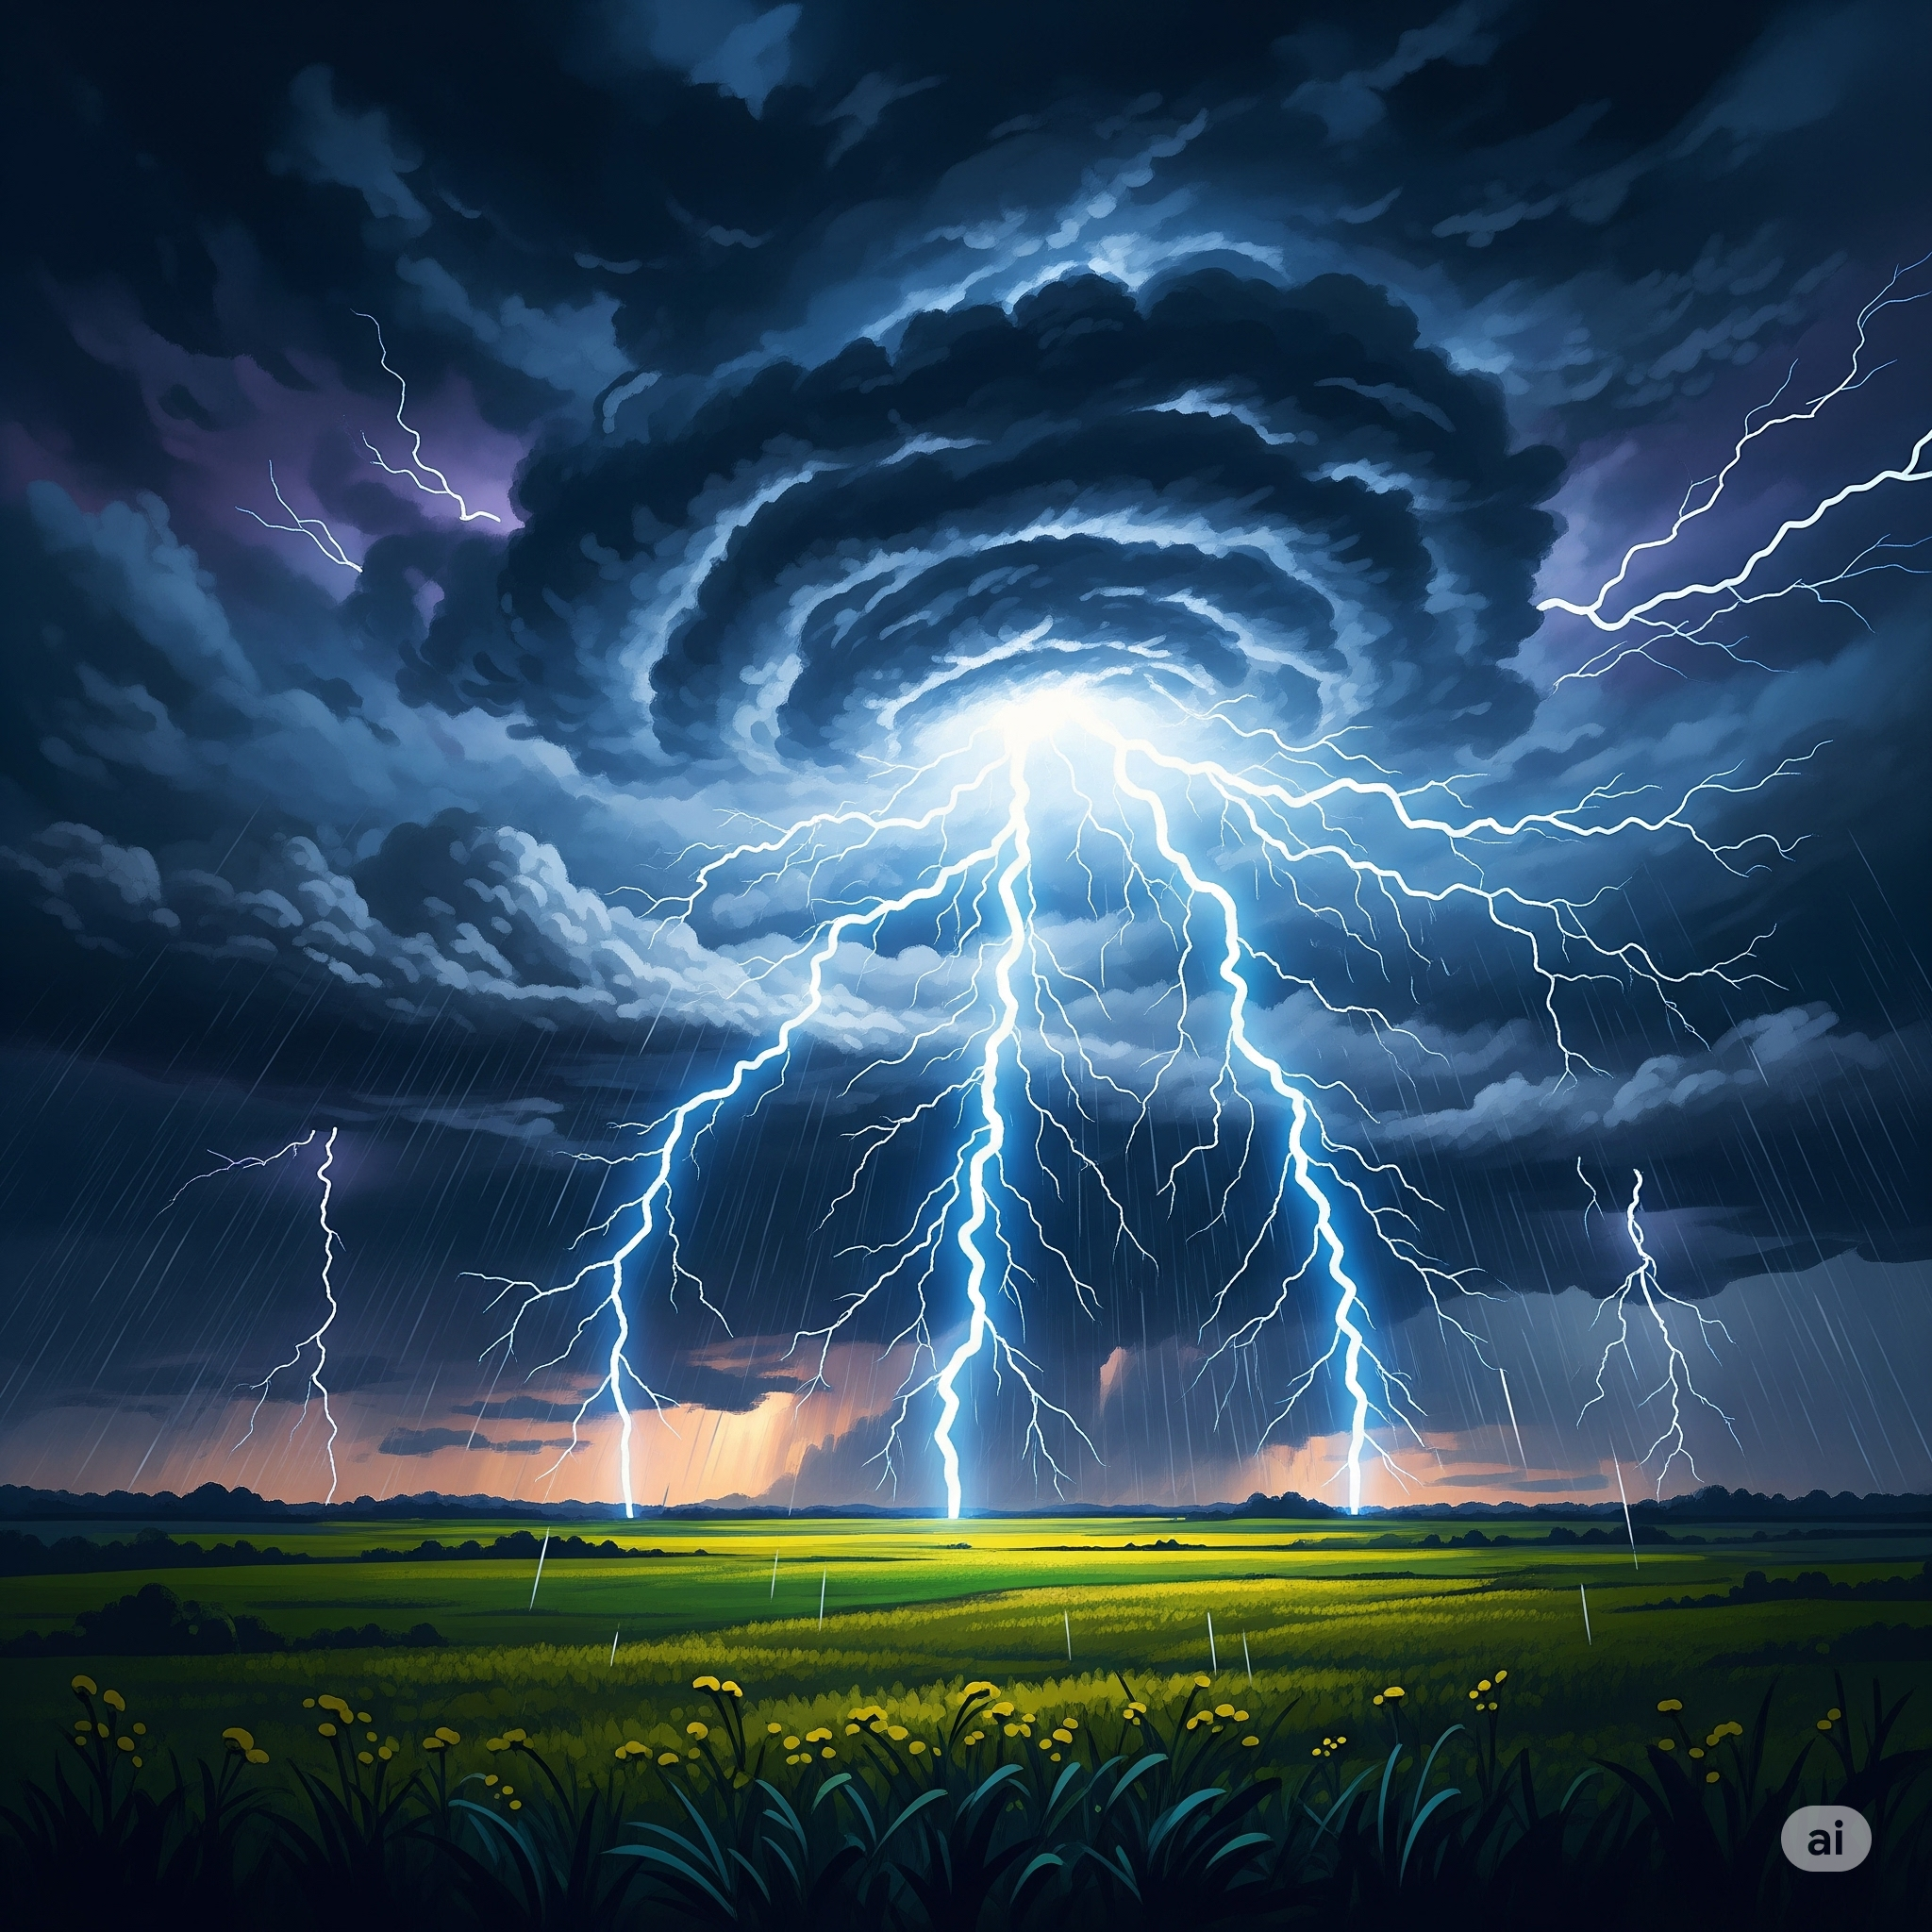
\includegraphics[width=5cm]{Images/anhhoa11/C02_B05_HC_VS_OXIGEN_CUA_NITROGEN/troi_giong.png}}
	\end{kd}
	%%%Phần lý thuyết
	\subsection{Nội dung bài học}
	\subsubsection{Các oxide của nitrogen và hiện tượng mưa acid}
	\Noibat[\maunhan][][][]{Nguồn gốc các oxide của nitrogen}
	\begin{ghinho}
		Trong tự nhiên và trong các hoạt động của con người, các oxide của nitrogen (thường được kí hiệu chung là $NO_x$) được tạo thành.
		\begin{enumerate}
			\item \textbf{Nitrogen monoxide (NO):} Là khí không màu, được tạo thành trong không khí ở nhiệt độ rất cao (khoảng $3000^\circ C$), ví dụ như khi có sấm sét. 
			\[\mathrm{N}_2(g) + \mathrm{O}_2(g) \xharpoonarrow[$3000^{\circ}C$] 2\mathrm{NO}(g)\]
			\item \textbf{Nitrogen dioxide ($NO_2$):} Ở điều kiện thường, khí NO không màu kết hợp nhanh với oxygen trong không khí tạo thành khí nitrogen dioxide ($NO_2$) có màu nâu đỏ, rất độc. 
			\[2\mathrm{NO}(g) + \mathrm{O}_2(g) \xrightarrow 2\mathrm{NO}_2(g)\]
		\end{enumerate}
	\end{ghinho}
	\begin{hoivadap}
		Dựa vào kiến thức về năng lượng liên kết của phân tử $N_2$ đã học, hãy giải thích tại sao phản ứng giữa nitrogen và oxygen chỉ xảy ra ở nhiệt độ rất cao hoặc khi có tia lửa điện?
	\end{hoivadap}
	\begin{Bancobiet}
		\immini{Ngoài nguồn gốc tự nhiên như sấm sét, các khí $NO_x$ còn phát sinh từ các hoạt động của con người, chủ yếu từ việc đốt cháy nhiên liệu ở nhiệt độ cao trong động cơ ô tô, nhà máy nhiệt điện, và các lò công nghiệp. Các khí này là một trong những nguyên nhân chính gây ô nhiễm không khí và các vấn đề môi trường. }{\includegraphics[width =5cm]{Images/anhhoa11/C02_B05_HC_VS_OXIGEN_CUA_NITROGEN/khithai.jpg}}
	\end{Bancobiet}
	\Noibat[\maunhan][][][]{Hiện tượng mưa acid}
    \begin{center}
	  \includegraphics[width =8cm]{Images/anhhoa11/C02_B05_HC_VS_OXIGEN_CUA_NITROGEN/mua_axit.jpg}
	  \captionof{figure}{Sơ đồ quá trình hình thành mưa acid}
    \end{center}
	\begin{tomtat}
		\textbf{Mưa acid} là hiện tượng nước mưa có độ pH thấp hơn 5,6. Nguyên nhân chủ yếu là do sự oxi hoá các khí $SO_2$ và các oxide của nitrogen ($NO_x$) có trong khí quyển, với sự xúc tác của các ion kim loại trong khói bụi, sau đó hoà tan vào nước mưa tạo thành dung dịch sulfuric acid ($H_2SO_4$) và nitric acid ($HNO_3$). 
		\[4\mathrm{NO}_2(g) + \mathrm{O}_2(g) + 2\mathrm{H}_2\mathrm{O}(l) \xrightarrow 4\mathrm{HNO}_3(aq)\]
	\end{tomtat}
	\Noibat[\maunhan][][][]{Tác hại của mưa acid}
	\begin{hopdongian}
		Mưa acid gây ra nhiều tác hại nghiêm trọng:
		\begin{itemize}
			\item \textbf{Đối với môi trường:} Phá huỷ rừng cây, làm thay đổi thành phần hoá học của đất và nước, gây hại cho các sinh vật sống trong sông, hồ. 
			\item \textbf{Đối với công trình:} Ăn mòn, phá huỷ các công trình kiến trúc làm từ đá vôi, đá cẩm thạch và các vật liệu kim loại. 
			\item \textbf{Đối với con người:} Gây ảnh hưởng tiêu cực đến sức khoẻ, đặc biệt là các bệnh về đường hô hấp. 
		\end{itemize}
	\end{hopdongian}
	
	\subsubsection{Nitric acid}
	\Noibat[\maunhan][][][]{Cấu tạo phân tử và tính chất vật lí}\\
		Phân tử nitric acid có công thức cấu tạo như hình (\ref{ctctnitric}).\\Trong phân tử $HNO_3$ nguyên tử N có số oxi hóa là $+5$:
		\begin{figure}[!htp]
			\begin{center}
				%% Hình phụ 1
				\subcaptionbox{\label{ctctnitric}}[5cm]{\chemfig[atom sep=4em]{H-[:-30]O-[:30]N(=[90,0.8]O)-[:-30,,,,->,>=stealth]O}}
				%% Hình phụ 2
				\subcaptionbox{\label{ctphantunitric}}[5cm]{\includegraphics[width=3cm]{Images/anhhoa11/C02_B05_HC_VS_OXIGEN_CUA_NITROGEN/nitric_acid_3d.png}}
				%% Hình phụ 3
				\subcaptionbox{\label{binhnitric}}[5cm]{\includegraphics[width=3.4cm]{Images/anhhoa11/C02_B05_HC_VS_OXIGEN_CUA_NITROGEN/nitric_acid.png}}
				\caption{Cấu tạo phân tử nitric acid (a), mô hình phân tử nitric acid (b), nitric acid được bảo quản trong lọ thủy tinh tối màu (c)}
			\end{center}
		\end{figure}
	\begin{ghinho}
		\textbf{Tính chất vật lí:}
		\begin{itemize}
			\item Nitric acid tinh khiết là chất lỏng, không màu, bốc khói mạnh trong không khí ẩm. 
			\item Kém bền, dễ bị phân hủy bởi ánh sáng tạo thành khí $NO_2$ màu nâu đỏ, làm cho dung dịch có màu vàng. [cite\_start]Do đó, cần được bảo quản trong lọ tối màu. 
			\[4HNO_3 \xrightarrow[as] 4NO_2 + O_2 + 2H_2O\]
			\item Tan vô hạn trong nước. Dung dịch nitric acid thương mại thường có nồng độ 68\%. 
		\end{itemize}
	\end{ghinho}
	
	\Noibat[\maunhan][][][]{Tính chất hóa học}
	\begin{tomtat}
		Nitric acid có hai tính chất hóa học đặc trưng là tính acid mạnh và tính oxi hóa rất mạnh.
		\begin{enumerate}
			\item \textbf{Tính acid mạnh:} Trong dung dịch, $HNO_3$ phân li hoàn toàn, thể hiện đầy đủ tính chất của một acid mạnh.
			\[\mathrm{HNO}_3 \xrightarrow \mathrm{H}^+ + \mathrm{NO}_3^-\]
			Tác dụng với base, basic oxide, và muối của acid yếu hơn.
			\begin{eqnarray*}
				HNO_3 + NaOH &\xrightarrow& NaNO_3 + H_2O \\
				2HNO_3 + CuO &\xrightarrow& Cu(NO_3)_2 + H_2O \\
				2HNO_3 + CaCO_3 &\xrightarrow& Ca(NO_3)_2 + CO_2\uparrow + H_2O
			\end{eqnarray*}
			\item \textbf{Tính oxi hóa mạnh:} Do có số oxi hóa $+5$ cao nhất, $HNO_3$ có khả năng oxi hóa được hầu hết các kim loại (trừ Au, Pt) và nhiều phi kim, hợp chất khác.  Tùy thuộc vào nồng độ acid và độ mạnh yếu của chất khử, sản phẩm khử của $N^{+5}$ có thể là $NO_2$, $NO$, $N_2O$, $N_2$, hoặc $NH_4NO_3$.
		\end{enumerate}
	\end{tomtat}
	\begin{Bancobiet}
		\immini{Hỗn hợp dung dịch $HNO_3$ đặc và $HCl$ đặc theo tỉ lệ thể tích 1:3 được gọi là \textbf{nước cường toan} (aqua regia). Hỗn hợp này có khả năng hòa tan được cả vàng (Au) và platinum (Pt), những kim loại không tan trong các acid thông thường.}{\includegraphics[width=5cm]{Images/anhhoa11/C02_B05_HC_VS_OXIGEN_CUA_NITROGEN/nuoc_cuong_toang.png}} 
	\end{Bancobiet}
	\Noibat[\maunhan][][][]{Ứng dụng}
	\begin{ghinho}
		Nitric acid là một trong những hóa chất cơ bản và quan trọng nhất trong công nghiệp, với nhiều ứng dụng:
		\begin{itemize}
			\item Sản xuất phân bón, đặc biệt là phân đạm (ví dụ: $NH_4NO_3$). 
			\item Sản xuất thuốc nổ, ví dụ như trinitrotoluene (TNT). 
			\item Sản xuất thuốc nhuộm, dược phẩm. 
		\end{itemize}
	\end{ghinho}
	\begin{hoivadap}
		Tại sao có thể dùng bình bằng nhôm (Al) hoặc sắt (Fe) để đựng dung dịch $HNO_3$ đặc, nguội mà không dùng để đựng dung dịch $HNO_3$ loãng? 
	\end{hoivadap}
	%%%%%%%%%
	\subsubsection{Hiện tượng phú dưỡng}
	\Noibat[\maunhan][][][]{Khái niệm và nguyên nhân}
	\begin{tomtat}
		\textbf{Phú dưỡng} (eutrophication) là hiện tượng ao, hồ bị dư thừa các nguyên tố dinh dưỡng, chủ yếu là Nitrogen (dưới dạng nitrate $NO_3^-$) và Phosphorus (dưới dạng phosphate $PO_4^{3-}$). 
	\end{tomtat}
	\begin{ghinho}
		\textbf{Nguyên nhân chính gây ra hiện tượng phú dưỡng:}
		\begin{itemize}
			\item Nước thải sinh hoạt, công nghiệp, và chăn nuôi chưa qua xử lí được thải trực tiếp vào nguồn nước. 
			\item Việc lạm dụng phân bón hóa học trong nông nghiệp, lượng phân bón dư thừa bị rửa trôi theo nước mưa xuống ao, hồ, sông, suối. 
		\end{itemize}
	\end{ghinho}
	\Noibat[\maunhan][][][]{Hệ quả và biện pháp khắc phục}
	\begin{hopdongian}
		\textbf{Hệ quả của phú dưỡng:}
		\begin{enumerate}
			\item \textbf{Tảo và thực vật thủy sinh phát triển mạnh:} Lượng dinh dưỡng dồi dào làm cho rong, tảo, bèo phát triển bùng nổ, che kín mặt nước, ngăn cản ánh sáng và oxy khuếch tán xuống các tầng nước sâu hơn. 
			\item \textbf{Suy giảm oxy hòa tan:} Khi tảo và thực vật chết đi, chúng bị vi khuẩn hiếu khí phân hủy. Quá trình này tiêu thụ một lượng lớn oxy hòa tan trong nước. 
			\item \textbf{Hủy diệt sinh vật:} Nồng độ oxy giảm đột ngột làm cho các loài động vật thủy sinh như cá, tôm chết hàng loạt, gây ô nhiễm nghiêm trọng và mất cân bằng hệ sinh thái. 
		\end{enumerate}
	\end{hopdongian}
	\begin{hoivadap}
		Để hạn chế hiện tượng phú dưỡng và bảo vệ môi trường nước, chúng ta cần thực hiện những biện pháp gì trong sinh hoạt và sản xuất nông nghiệp? 
	\end{hoivadap}
	